To classify different types of image sequences MLpy library was used. MLpy is a machine learning library for python which provides a variety of algorithms and tools to perform machine learning on data.

The algorithm used in this project is Linear Support Vector Machine which was trained over 5 principal components of the input data. Methods of producing such data was further described in Section \ref{sec:extraction}.

\subsubsection*{Principal Component Analysis}

Input vector consists of 12 features for every image sequence - 7 Hu moments and 5 area measures over time, therefore dataset lies in 12 dimensional space. principal component analysis (PCA) was performed on the input dataset to reduce dimensionality of the dataset. Prior to PCA all the features are normalised the zero mean and unit standard deviation. Figure \ref{fig:pcaplot} shows that first 5 principal components can explain most of the variance of the dataset. Therefore, we can deduct that input data sits on a five dimensional manifold. 

Using these components we project entire dataset as well as any new input data into 5 dimensional subspace.

\begin{figure}[htp]
\begin{center}
\leavevmode
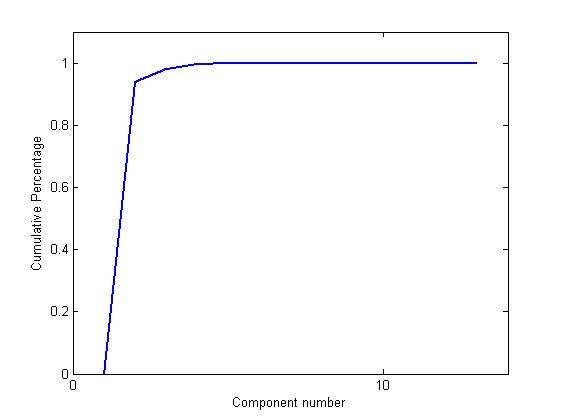
\includegraphics[width=0.6\textwidth] {pca.jpg}
\end{center}
\caption{Cumulative Percentage PCs}
\label{fig:pcaplot}
\end{figure}

\subsubsection*{Support Vector Machine}

Projected data is then used to train a linear support vector machine (SVM). The algorithm used is an implementation of multi-class support vector classification by Crammer and Singer. This algorithm is also available in MLpy library.

Logistic regression was also tested. However, as results in Section \ref{sec:results} shows SVM outperformed logistic regression and therefore was chosen to be used in the project. 

\subsubsection*{Cross Validation}

In order to evaluate performance of the classifier we utilised Leave-One-Out Cross-Validation. At each step the algorithm takes one instance of the data and performs training on the remaining data. Accuracy of prediciting left out data point is used as an evaluation metric. Using the trained classifier test instances are checked and results averaged for entire dataset.

Summary of the algorithms and parameters used in the classification module is presented in table \ref{tbl:classification}.

\begin{table}
\begin{tabular}{|c|l|}
\hline 
Preprocessing: & 1.  Feature Normalization, zero mean standard deviation\\ 
& 2. Principal Component Analysis with 5 Components\\
\hline 
Training Algorithm & Multi-class SVM \\ 
\hline 
Performance Measure & Leave-One-Out Cross-Validation \\ 
\hline 

\end{tabular} 
\caption{Summary of classification module parameters and algorithms}
\label{tbl:classification}
\end{table}